\documentclass[10pt]{article}
\usepackage[margin=0.85in]{geometry}
\usepackage{amsmath,amssymb,booktabs,graphicx,caption}
\usepackage[hidelinks]{hyperref}
\captionsetup{font=small}
\setlength{\tabcolsep}{4pt}

\title{The $J_1$--$J_2$ model on $4\times L_x$ cylinders:\\ inputs, trial states, costs and crossover}
\author{Data report for the filter-pipeline paper}
\date{\today}

\begin{document}
\maketitle

\noindent This report collects every two-dimensional result produced for the paper. All tables and figures are
generated by \texttt{sbpipe\_study/report2d/make\_report2d.py} from \texttt{sbpipe\_study/results/*.json}
(\texttt{ext\_inputs2d.json}, \texttt{cache2d/}, \texttt{ext\_regime\_cyl*.json}, \texttt{emp\_regime.json},
\texttt{emp\_frontier.json}). Nothing in it is typed by hand.

\section{Model and pipeline settings}

\begin{equation}
H=J_1\sum_{\langle ij\rangle}\mathbf S_i\cdot\mathbf S_j+J_2\sum_{\langle\langle ij\rangle\rangle}\mathbf S_i\cdot\mathbf S_j,
\qquad J_1=1,
\end{equation}
on an $L_x\times4$ square lattice, periodic around the four-site circumference and open along $L_x=3,4,6,8,12$
($N=12$--48 qubits), at $J_2=0$ and $0.3$. Site $(x,y)$ is qubit $4x+y$, so the MPS runs up each column in
turn (a snake path). $J_2=0.5$ is left out because ED on $4\times4$ shows that its lowest excitation is not the
triplet, while the pipeline takes $E_1$ as the lowest $S^z=1$ state.

\begin{itemize}
\item \textbf{Energies.} DMRG (quimb) with reference bond dimensions $\chi=16,\dots,256$. $E_0$ and $E_1$ (the
lowest $S^z=1$ state) are taken from $\chi=256$, with the error estimated from the last change in $\chi$. The
spectral upper bound is Weyl's. ED is run for $4\times3$ and $4\times4$.
\item \textbf{Trial states.} Variational MPS at $\chi=2,\dots,64$. The overlap $\gamma=|\langle E_0|\psi_\chi\rangle|^2$
is measured against the $\chi=256$ reference (or ED). Each trial is costed as a staircase of
quantum-Shannon-decomposed unitaries.
\item \textbf{Filter.} QETU (Chebyshev) or the dyadic/optimized cosine filters, second-order Strang steps,
CNOT counts from Pauli-gadget ladders. \emph{Certified} costs come from the pipeline's a-priori
bound. \emph{Empirical} costs use the two laws measured on exact spectra for $N\le16$ (675 cases): the
smallest working degree is $d\,\Delta\simeq(2/\pi)\cosh^{-1}(1/\eta)$ with $\eta^2=\gamma\epsilon/(1-\gamma)$, and one
Strang step per query suffices.
\end{itemize}

\section{Energies and gaps}

\begin{table}[h]
\centering\small
\caption{Inputs per cylinder. $E_0$, $E_1$ from DMRG at $\chi\le256$; the errors are the pipeline inputs.
$E_{\max}$ is the Weyl upper bound, ``time'' is the wall-clock DMRG time in hours, and the last column gives
$|E^{\rm DMRG}-E^{\rm ED}|$ for $E_0$ and $E_1$ where ED is available.}
\begin{tabular}{lrrrrrrrrrc}
\toprule
system & $N$ & $J_2$ & $E_0$ & $E_1$ & gap & $\delta E_0$ & $\delta E_1$ & $E_{\max}$ & time [h] & ED check \\
\midrule
@@TAB_INPUTS@@
\bottomrule
\end{tabular}
\end{table}

The triplet gap closes slowly with $L_x$: from 0.66 to 0.35 at $J_2=0$ and from 0.73 to 0.51 at $J_2=0.3$
(Fig.~\ref{fig:inputs}c). Frustration opens the finite-size gap here. Because the Weyl bound grows as $N$, the
scaled gap $\Delta=g/W$ that sets the filter degree falls roughly as $1/N$. The DMRG energy errors grow
from $10^{-10}$ ($4\times3$, exact at $\chi=64$) to $2$--$5\times10^{-4}$ at $4\times12$. Where ED exists, DMRG matches it to
$10^{-11}$ or better.

\begin{table}[h]
\centering\small
\caption{DMRG convergence of $E_0$: $|E_0(\chi)-E_0(256)|$.}
\begin{tabular}{lrccccc}
\toprule
system & $J_2$ & $\chi=16$ & 32 & 64 & 128 & 256 \\
\midrule
@@TAB_CONV@@
\bottomrule
\end{tabular}
\end{table}

\begin{figure}[h]
\centering
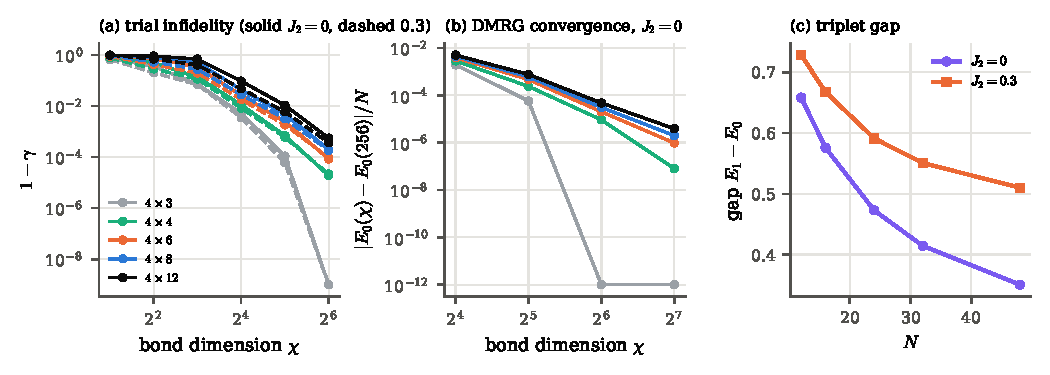
\includegraphics[width=\textwidth]{figs/fig_inputs.pdf}
\caption{(a) Trial infidelity $1-\gamma$ versus bond dimension for every cylinder (solid $J_2=0$, dashed $J_2=0.3$).
(b) DMRG energy convergence per site. (c) Triplet gap versus $N$.}
\label{fig:inputs}
\end{figure}

\section{Trial states: overlap and circuit cost}

\begin{table}[h]
\centering\small
\caption{Trial infidelity $1-\gamma$ of the variational MPS. Values at the $10^{-4}$ level and below for
$L_x\ge8$ are limited by the accuracy of the $\chi=256$ reference.}
\begin{tabular}{lrcccccc}
\toprule
system & $J_2$ & $\chi=2$ & 4 & 8 & 16 & 32 & 64 \\
\midrule
@@TAB_OVERLAP@@
\bottomrule
\end{tabular}
\end{table}

\begin{table}[h]
\centering\small
\caption{CNOTs of the MPS preparation circuit (independent of $J_2$).}
\begin{tabular}{lcccccc}
\toprule
system & $\chi=2$ & 4 & 8 & 16 & 32 & 64 \\
\midrule
@@TAB_COST@@
\bottomrule
\end{tabular}
\end{table}

Compared with the chain, the snake MPS converges much more slowly in $\chi$. The 48-site chain reaches
$1-\gamma\le10^{-2}$ at $\chi=8$; the $4\times12$ cylinder needs $\chi=32$ for the same, and $\chi=64$ leaves
$5.5\times10^{-4}$ ($J_2=0$). The trial cost grows as $\chi^2N$, so each doubling of $\chi$ costs about $4\times$.
That combination (slow convergence, quadratic cost) is what opens room for the filter.

\section{Cheapest route to a fixed target}

Table~\ref{tab:regime} compares three routes at $\epsilon=10^{-2},10^{-3},10^{-4}$:
\begin{itemize}
\item the cheapest MPS that meets $1-\gamma\le\epsilon$ on its own;
\item the cheapest certified filtered plan (any $\chi$; dyadic, optimized or QETU);
\item the cheapest empirical filtered plan (QETU at the degree law, one step per query).
\end{itemize}
Filtered costs are expected CNOTs per success, including the trial circuit on every attempt.

\begin{table}[h]
\centering\footnotesize
\caption{CNOTs (bond dimension in parentheses). M: MPS alone. C: certified filter. E: empirical filter.
``--'': no $\chi\le64$ route.}
\label{tab:regime}
\resizebox{\textwidth}{!}{%
\begin{tabular}{lr ccc ccc ccc}
\toprule
 & & \multicolumn{3}{c}{$\epsilon=10^{-2}$} & \multicolumn{3}{c}{$\epsilon=10^{-3}$} & \multicolumn{3}{c}{$\epsilon=10^{-4}$}\\
\cmidrule(lr){3-5}\cmidrule(lr){6-8}\cmidrule(lr){9-11}
system & $J_2$ & M & C & E & M & C & E & M & C & E \\
\midrule
@@TAB_REGIME@@
\bottomrule
\end{tabular}}
\end{table}

\paragraph{Certified.} The certified filter never beats a compiled MPS that reaches the target, usually missing by
one to two orders of magnitude. It is the only route at $\epsilon=10^{-4}$ on $4\times8$ and $4\times12$, where no
$\chi\le64$ trial suffices. Its excess comes almost entirely from the Trotter bound, which asks for about
16 steps per query where one is enough.

\paragraph{Empirical.} With the measured filter cost the comparison depends on where the target falls on the
MPS staircase. The empirical filter wins whenever the target lies just beyond what the current $\chi$ reaches, so that
the MPS would need the next doubling: for example $4\times4$ at $10^{-2}$ and $10^{-4}$, $4\times6$ and $4\times8$ at
$10^{-3}$, and $4\times12$ at $10^{-2}$ ($J_2=0$). Otherwise it loses, by up to $6\times$ (e.g. $4\times12$, $J_2=0.3$,
$10^{-2}$, where $\chi=32$ already suffices). It is the only route at $10^{-4}$ on $4\times8$ and $4\times12$.

\paragraph{Check of the empirical laws.} For $4\times3$ and $4\times4$ (and the 16-site chain) the trial
state vectors are available. There we ran the actual QETU circuit, one Strang step per query, at the degree
the law predicts. In @@NOK@@ of @@NSIM@@ cases it met the target at exactly that degree
(Table~\ref{tab:sim}).

\begin{table}[h]
\centering\small
\caption{State-vector simulation of the empirical filter on cylinders: predicted degree, degree that
reached $\epsilon$ with one Strang step per query, measured infidelity and success probability.}
\label{tab:sim}
\begin{tabular}{lrrrcrrcc}
\toprule
system & $J_2$ & $\chi$ & $\gamma$ & $\epsilon$ & $d$ (law) & $d$ (sim) & $1-F$ & $p$ \\
\midrule
@@TAB_SIM@@
\bottomrule
\end{tabular}
\end{table}

\section{Cost per accuracy and the crossover}

For a continuous view we compute the cheapest cost to reach every infidelity between $10^{-1}$ and $10^{-7}$
(Fig.~\ref{fig:cross}):
\begin{itemize}
\item MPS alone: the cheapest $\chi$ with $1-\gamma\le\epsilon$, a staircase in $\epsilon$;
\item the empirical filter: minimized over the trial $\chi$;
\item the certified filter: at the three targets above.
\end{itemize}

\begin{figure}[h]
\centering
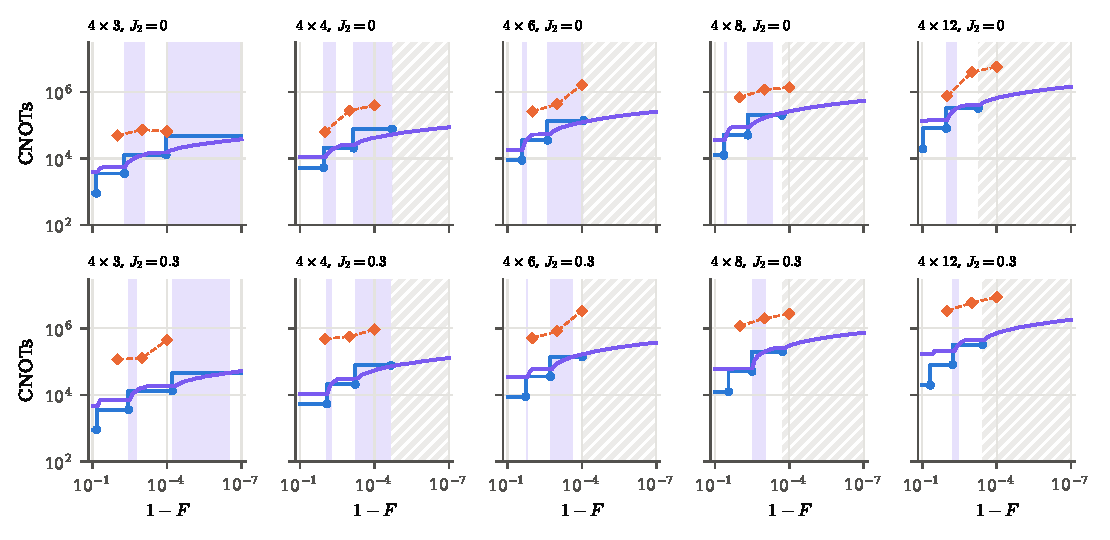
\includegraphics[width=\textwidth]{figs/fig_crossover2d.pdf}
\caption{Cheapest CNOTs to reach infidelity $1-F$ (accuracy increases to the right). Blue: MPS alone (dots are the
$\chi=2,\dots,64$ trials). Purple: MPS + filter, empirical. Orange diamonds: MPS + filter, certified. Purple
shading: the empirical filter is cheaper. Grey hatching: no MPS with $\chi\le64$ reaches that accuracy.}
\label{fig:cross}
\end{figure}

\begin{table}[h]
\centering\small
\caption{Accuracy windows in which the empirical filter is cheaper than any MPS that meets the target alone
(largest saving in parentheses; windows narrower than a factor 1.5 in $1-F$ omitted), and the accuracy
beyond which no $\chi\le64$ MPS suffices.}
\begin{tabular}{lrlc}
\toprule
system & $J_2$ & filter cheaper for $1-F$ in & MPS ($\chi\le64$) limit \\
\midrule
@@TAB_CROSS@@
\bottomrule
\end{tabular}
\end{table}

\paragraph{Reading the crossover.} On every cylinder the empirical filter wins in the accuracy window just
before the MPS needs its next doubling of $\chi$: a short filter on the current $\chi$ is cheaper than a
$4\times$ larger trial circuit. The saving in that window is a factor of 2--3. Two trends follow from the inputs:
\begin{itemize}
\item The window moves to looser accuracy as the cylinder grows (from around $10^{-4}$ at $4\times4$ to around
$10^{-2}$ at $4\times12$). Each $\chi$ buys less overlap on a longer cylinder, while the filter degree depends on
the overlap only logarithmically.
\item Beyond the MPS limit ($2\times10^{-5}$ at $4\times4$, $5\times10^{-4}$ at $4\times12$) the filter is the only
route in our data. A $\chi=128$ trial would cost about $4\times$ the $\chi=64$ one, roughly $1.3\times10^{6}$ CNOTs at
$4\times12$, about what the empirical filter needs for $1-F=10^{-6}$ and more than it needs at any looser target, even if such a trial reached that accuracy.
\end{itemize}
The chain has no such crossover (see the regime section of the paper): its MPS overlap converges fast enough in $\chi$ that the next
doubling is always the cheaper option.

\section{Caveats}
\begin{itemize}
\item The empirical filter cost rests on two laws measured for $N\le16$ (chain and the two small cylinders).
They held in every case we could simulate, but beyond $N=16$ they are extrapolated, and they are not a
certificate. Only the certified curve carries a guarantee, and it does not cross the MPS.
\item Overlaps at the $10^{-4}$ level and below for $L_x\ge8$, and energy errors of $2$--$5\times10^{-4}$ at $4\times12$,
are limited by the $\chi=256$ DMRG reference. The MPS staircase is therefore uncertain at its tight end on
the larger cylinders.
\item ED confirms the triplet as the first excitation only for $4\times3$ and $4\times4$. For larger cylinders
this is an assumption.
\item Costs are CNOT counts with all-to-all connectivity. Trial circuits use a generic decomposition bound,
not compiled circuits. Repeat-until-success is assumed throughout.
\item Only width-4 cylinders were studied. Wider cylinders, where the snake MPS degrades faster, are the
natural next test of whether the crossover window widens.
\end{itemize}

\end{document}
